\appendix

\section{Design choices, tested}
\label{app:design}

Four choices in Section~\ref{sec:method_model} could each have been made the other way. Each is ablated with everything else held fixed.

\subsection{The gate is smooth, and one-sided}

A step gate, $\mathbf{1}[\Delta<\tau]$, zeroes $\zmix$'s gradient outright beyond the threshold rather than passing a partial one. It is worse on both stems (Table~\ref{tab:gatehard}). Since $\tau$ cannot be chosen accurately without labels (Section~\ref{sec:handpicked}), horizons near it should not flip between fully passed and fully blocked under the smallest movement of the threshold; the width $\kappa$ is what gives them intermediate values, and it earns its place.

\begin{table}[!tb]
\caption{A step gate against the smooth one. The smooth gate is
$g(\Delta)=\sigma((\tau-\Delta)/\kappa)$; the step version replaces it with
$\mathbf{1}[\Delta<\tau]$, which zeroes $\zmix$'s gradient outright beyond $\tau$
instead of passing a partial one. Cells are SEP on synthetic, $n=5$ seeds, all else
held fixed. The step form is worse on both stems, which is why $\tau$'s width
$\kappa$ is part of the method rather than a smoothing convenience.}
\label{tab:gatehard}
\centering
\small
\begin{tabular}{lccc}
\hline
Stem & Smooth gate (ours) & Step gate & Difference \\
\hline
HGLP-Reg & \textbf{0.408} & 0.353 & $-0.056$ \\
HGLP-NCE & \textbf{0.749} & 0.684 & $-0.066$ \\
\hline
\end{tabular}
\end{table}


The symmetric variant multiplies $\zslow$ by $1-g(\Delta)$, switching it off below $\tau$ so that no horizon can deposit transient information in it. This is the obvious structural way to buy the exclusion the objective cannot enforce, and it does not work: it is better in \numSymBetter{} of six settings and worse in \numSymWorse{} (Table~\ref{tab:gatesym}), costing $\numSymWorstDrop$ SEP on the synthetic regression stem. Removing $\zslow$ from the near horizons removes its training signal there as well, and the block loses more from being untrained than it gains from being protected --- which is the argument of Section~\ref{sec:asymmetry}, now measured.

\begin{table}[!tb]
\caption{Can exclusion be bought structurally? The symmetric variant multiplies
$\zslow$ by $1-g(\Delta)$, switching it off below $\tau$ so that no horizon can push
transient information into it. Cells are SEP at each model's own best $\lambda$ over
$\{0,1,4,16,64\}$, $n=5$ seeds; higher is better; differences within $\pm0.005$ SEP
are called a tie. The asymmetric gate of Eq.~\ref{eq:gate} is better in 4 of
6 settings against 1 for the symmetric one, so the design choice is not
an oversight.}
\label{tab:gatesym}
\centering
\small
\begin{tabular}{llcccc}
\hline
Dataset & Stem & Asymmetric (ours) & Symmetric & Difference & Better \\
\hline
Synthetic & HGLP-Reg & 0.814 ($\lambda=1$) & 0.673 ($\lambda=1$) & $-0.141$ & asym \\
Synthetic & HGLP-NCE & 0.849 ($\lambda=16$) & 0.873 ($\lambda=4$) & $+0.024$ & \textbf{sym} \\
PTB-XL & HGLP-Reg & 0.495 ($\lambda=4$) & 0.438 ($\lambda=1$) & $-0.057$ & asym \\
PTB-XL & HGLP-NCE & 0.567 ($\lambda=4$) & 0.567 ($\lambda=16$) & $-0.000$ & tie \\
HAPT & HGLP-Reg & 0.677 ($\lambda=1$) & 0.575 ($\lambda=4$) & $-0.102$ & asym \\
HAPT & HGLP-NCE & 0.626 ($\lambda=64$) & 0.598 ($\lambda=64$) & $-0.028$ & asym \\
\hline
\end{tabular}
\end{table}


\subsection{The target's receptive field is bounded}

The gate rests on a premise: withholding $\zmix$ at long range should cost nothing, because the transient factor is already forgotten there. That premise is a property of the data \emph{and of how the target is defined}, so it can be measured directly. For each horizon we fit two linear readings of the target embedding, one from the persistent factor alone and one from both factors, and take the difference (Table~\ref{tab:targetpilot}).

\begin{table}[!tbp]
\caption{Is withholding the transient block harmless at long range? Cells are
$R^2(s,u\!\to\!\bar z_{t+\Delta}) - R^2(s\!\to\!\bar z_{t+\Delta})$: how much the
transient factor adds, \emph{beyond} what the persistent factor already explains, to a
linear reading of the target embedding $\Delta$ ahead. \textbf{Zero means the transient
factor is redundant there}, so gating it away costs nothing. Synthetic, HGLP-Reg, 2{,}500
steps, one seed, ground-truth factors. The bounded target reaches zero at
$\Delta=16$ --- the value of $\tau$ used on this data --- and stays there; the cumulative
target never does, because its receptive field runs back to the start of the window and so
re-contains the anchor's own transient state. This is the measurement behind the
receptive-field bound of Eq.~\ref{eq:target}. It reads the target embedding rather than
downstream error, and it is one seed on one dataset.}
\label{tab:targetpilot}
\centering
\small
\begin{tabular}{lccccccccc}
\hline
Target $\Delta$ & 8 & 12 & 16 & 24 & 32 & 48 & 64 & 96 & 128 \\
\hline
Bounded (ours) & +0.103 & +0.025 & +0.003 & -0.001 & -0.000 & +0.000 & -0.001 & -0.000 & -0.000 \\
Cumulative & +0.024 & +0.022 & +0.024 & +0.020 & +0.017 & +0.013 & +0.011 & +0.008 & +0.008 \\
\hline
\end{tabular}

\medskip
\small On the same two runs, the bounded target also leaves less of the transient factor
in $\zslow$ ($R^2$ 0.041 against 0.660) and does not partially
collapse (target RankMe 12.9 against 5.3).
\end{table}


\begin{figure}[!tbp]
\centering
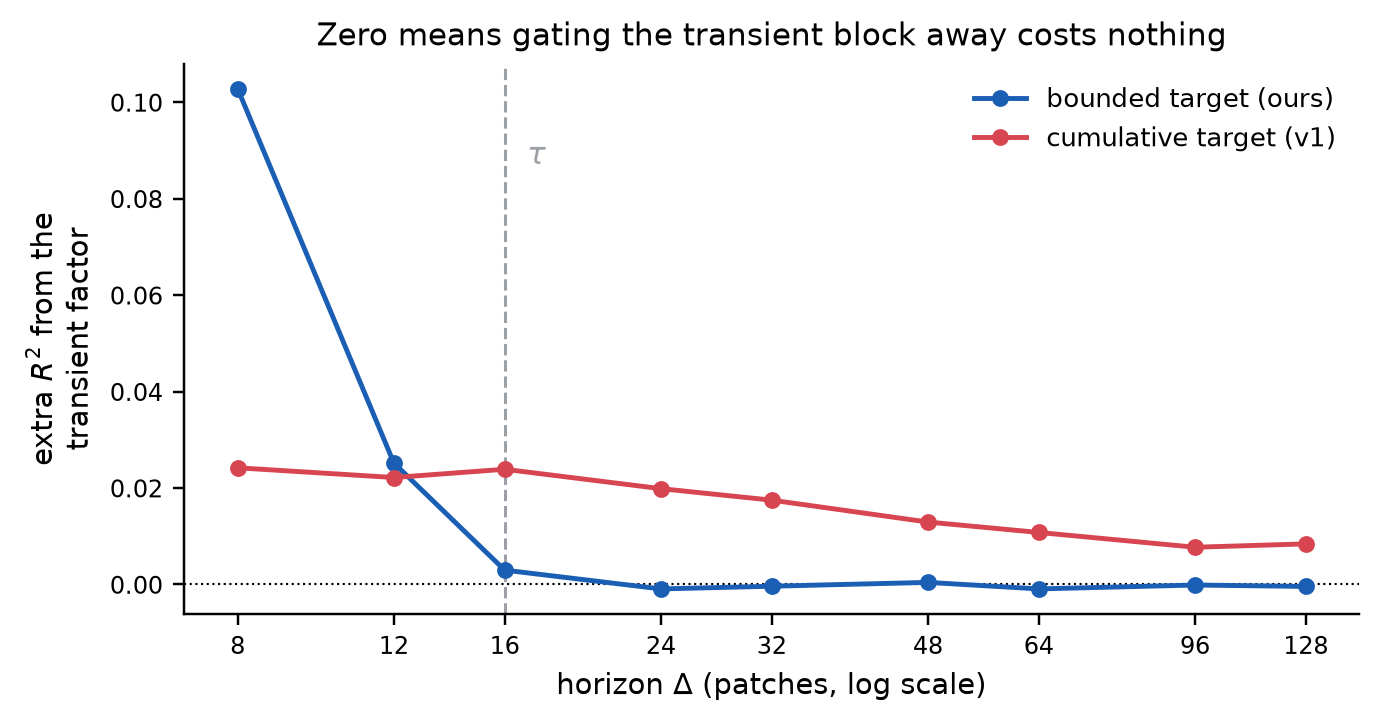
\includegraphics[width=0.72\textwidth]{figs/fig_target_pilot.png}
\caption{The same measurement as Table~\ref{tab:targetpilot}, as a curve. The bounded target falls to zero by $\Delta=\tau$ and stays there, so beyond the threshold the transient factor explains nothing about the target that the persistent factor does not already explain --- which is what makes gating it away harmless. The cumulative target of the earlier design stays above zero at every horizon, including the longest: its receptive field reaches back to the start of the window and so re-contains the anchor's own transient state, and no horizon is far enough to escape that.}
\label{fig:targetpilot}
\end{figure}

With the receptive-field bound of Eq.~\ref{eq:target} the difference reaches zero at $\Delta=16$ and stays there. With the cumulative target of the earlier design --- the causal encoder simply read at $t+\Delta$ --- it never reaches zero at any horizon, because that target's receptive field runs back to the start of the window and therefore re-contains the anchor's own transient state. The shortcut is closed by the bound, not by hope.

Two limits on how far this may be read. It measures what explains the \emph{target embedding}, not downstream error, and it reports only the \emph{increment} the transient factor adds over the persistent one, so it does not by itself establish that the persistent factor explains the target well. And it is one seed on one dataset, with ground-truth factors that only synthetic data provides.

\subsection{The target is latent, not raw}

This ablates the premise of the latent-prediction family: that prediction should be made in a latent space rather than on the raw signal. Gate, anchor, horizon and loss form are held fixed and only the prediction target changes. The latent target is the 64-dimensional output the target encoder reads from the future interval; the raw target is the patch itself at that time, with one extra linear head. Both models carry the cross-covariance penalty, so $\lambda$ means the same for each, and each is compared at its own best value.

\begin{table}[!tbp]
\caption{Latent target against raw target. Cells are SEP on synthetic, $n=5$ seeds, each stem at its own best $\lambda$. Bold marks the latent target. Everything but the prediction target is held fixed.}
\label{tab:latentraw}
\centering
\small
\begin{tabular}{lccc}
\hline
Stem & Latent (best) & Raw (best) & Difference \\
\hline
HGLP-Reg & \textbf{0.809} ($\lambda=1$) & 0.415 ($\lambda=4$) & $+0.394$ ($1.95\times$) \\
HGLP-NCE & \textbf{0.844} ($\lambda=16$) & 0.432 ($\lambda=16$) & $+0.411$ ($1.95\times$) \\
\hline
\end{tabular}
\end{table}

Predicting raw patches halves SEP on both stems (Table~\ref{tab:latentraw}). The allocation term is the same for the two targets, at 0.86 to 0.89, and the gap opens in inclusion: the raw target loses the persistent factor as the penalty grows, falling from 0.807 to 0.401, whereas the latent target stays above 0.97 throughout. The raw signal still contains the transient component, and the pressure to predict that too pushes the persistent factor out. The gate and the penalty are thus not sufficient on their own; the latent target has to be present as well.

\section{Is the persistent factor in the slow band of the signal?}
\label{app:coincidence}

Section~\ref{sec:rotation} attributes SFA's lead on real data to persistence and slowness
mostly coinciding there. One half of that can be checked directly on the raw signal: we
filter it to one band at a time and fit the same linear probe on that band alone
(Table~\ref{tab:bandaccess}).

\begin{table}[!tbp]
\caption{Is the persistent factor readable from the \emph{slow band of the signal}?
Each row filters the raw signal to one band at a time and fits the same linear probe on
that band alone. Cells are the score named in the second column; ``low band'' is
$0$--$0.5$\,Hz for HAPT (a true low-pass, keeping DC), $0.05$--$0.5$\,Hz for PTB-XL
(band-pass: the ECG baseline is arbitrary), $f<0.02$ for the synthetic carrier. The
ratio column is low band over chance. Only HAPT clears chance by a real margin.}
\label{tab:bandaccess}
\centering
\small
\begin{tabular}{llcccc}
\hline
Dataset & Score & Low band & Chance & Low/chance & Best band (score) \\
\hline
Synthetic & $R^2$ & $8.2\times 10^{-6}$ & 0 & --- & carrier freq.\ (0.279) \\
PTB-XL & macro-F1 & 0.498 & 0.500 & 1.00 & 2.0-5.0\,Hz (0.761) \\
HAPT & macro-F1 & \textbf{0.570} & 0.167 & \textbf{3.42} & 0.0-0.5\,Hz (0.570) \\
\hline
\end{tabular}
\end{table}


Only HAPT clears chance by a real margin, at $\numHaptBandRatio\times$, which is
unsurprising --- posture is the DC distribution of gravity across three accelerometer
axes. On PTB-XL the low band is \emph{at} chance (\numPtbLowBand{} against
\numPtbChance) and the diagnosis lives instead in the 2--5\,Hz QRS morphology, yet SFA
still leads there. So on PTB-XL the coincidence is not one of signal band, and what SFA
exploits instead is that the diagnosis is constant within a record, which makes its time
derivative zero --- the limiting solution of the quantity SFA maximizes. The two real
datasets are therefore won by two different routes, and the synthetic data, where the
factor is neither band-slow nor window-constant, is closed to both.

\section{Term decomposition and the non-linear probe}
\label{app:probe}

\begin{table}[H]
\caption{Where the shortfall against SFA sits. Cells are \emph{ours minus SFA} on one
term of SEP, paired by seed then averaged, $n=5$; positive means we lead, and our column is
taken at the listed $\lambda$.}
\label{tab:terms}
\centering
\small
\begin{tabular}{lllcccc}
\hline
Dataset & Stem & $\lambda$ & Inclusion & Allocation & Exclusion & SEP \\
\hline
Synthetic & HGLP-Reg & 1 & $+0.102$ & $+0.236$ & $+0.156$ & $+0.395$ \\
Synthetic & HGLP-NCE & 16 & $-0.006$ & $+0.327$ & $+0.266$ & $+0.451$ \\
PTB-XL & HGLP-Reg & 4 & $-0.007$ & $+0.048$ & $\mathbf{-0.136}$ & $-0.073$ \\
PTB-XL & HGLP-NCE & 4 & $-0.000$ & $+0.007$ & $\mathbf{-0.051}$ & $-0.031$ \\
HAPT & HGLP-Reg & 1 & $-0.033$ & $-0.011$ & $-0.007$ & $-0.039$ \\
HAPT & HGLP-NCE & 64 & $-0.041$ & $+0.155$ & $-0.016$ & $+0.100$ \\
\hline
\end{tabular}
\end{table}


Table~\ref{tab:terms} splits SEP into its three factors and pairs by seed. Inclusion is a draw everywhere; every real-data loss against SFA is a loss on exclusion alone, and every win is a win on allocation. This matches the design rather than surprising it --- the objective enforces availability and cannot enforce absence (Section~\ref{sec:gate}), and it is on that term, and only that term, that the method falls behind.

\begin{table}[H]
\caption{What survives a non-linear reader. The features, the splits and the blocks are
held fixed and only the probe head changes, from a linear model to a one-hidden-layer
MLP (256 units); the \emph{same} head is given to SFA, PCA and ICA, so no method is
tested more harshly than another. $\lambda=4$, one seed. \textbf{(a)} Cells are
$\text{MLP}-\text{linear}$ on one SEP term, averaged over four methods $\times$ six
settings. Only exclusion falls, and it is the term the objective never enforced.
\textbf{(b)} Cells are SFA's exclusion minus ours, so positive means SFA holds the
lead; the diagnosis of Table~\ref{tab:terms} was not an artifact of linear probing.}
\label{tab:mlpprobe}
\centering
\small
(a) Change in each SEP term when the probe head stops being linear\\[2pt]
\begin{tabular}{lcccc}
\hline
SEP term & Mean change & Worst & Best & Rows \\
\hline
Inclusion & $+0.015$ & $-0.027$ & $+0.113$ & 16 \\
Allocation & $+0.087$ & $+0.031$ & $+0.156$ & 16 \\
Exclusion & $-0.149$ & $-0.530$ & $+0.019$ & 16 \\
\hline
\end{tabular}

\medskip
(b) Exclusion gap, SFA minus ours\\[2pt]
\begin{tabular}{lcc}
\hline
Setting & Linear probe & MLP probe \\
\hline
PTB-XL/HGLP-Reg & $+0.085$ & $+0.122$ \\
PTB-XL/HGLP-NCE & $+0.020$ & $+0.033$ \\
HAPT/HGLP-Reg & $+0.009$ & $+0.236$ \\
HAPT/HGLP-NCE & $+0.000$ & $+0.000$ \\
\hline
\end{tabular}
\end{table}


Table~\ref{tab:mlpprobe} replaces the linear reading head with a one-hidden-layer MLP, giving the same head to every method. Part (a) reports the change in each SEP term: exactly one collapses, and it is exclusion. Part (b) reports SFA's exclusion lead under both heads: it survives, and in two settings widens, so the diagnosis of Table~\ref{tab:terms} was not an artifact of linear probing. PCA and ICA degrade sharply under the same head while SFA does not, which is worth noting on its own --- the baseline we trail is a robust one.

Three cautions. Because exclusion falls monotonically as the reading head grows, only comparisons made under a fixed head are meaningful; the absolute value is a property of the probe as much as of the embedding. We tried one hidden width, 256, and did not trace the curve. And this experiment fixes $\lambda=4$ with one seed, whereas Table~\ref{tab:terms} takes each setting at its own best $\lambda$, so cells of the two tables must not be read against each other.

\section{Reading $\zslow$ as a trajectory}
\label{app:traj}

\begin{figure}[!tbp]
\centering
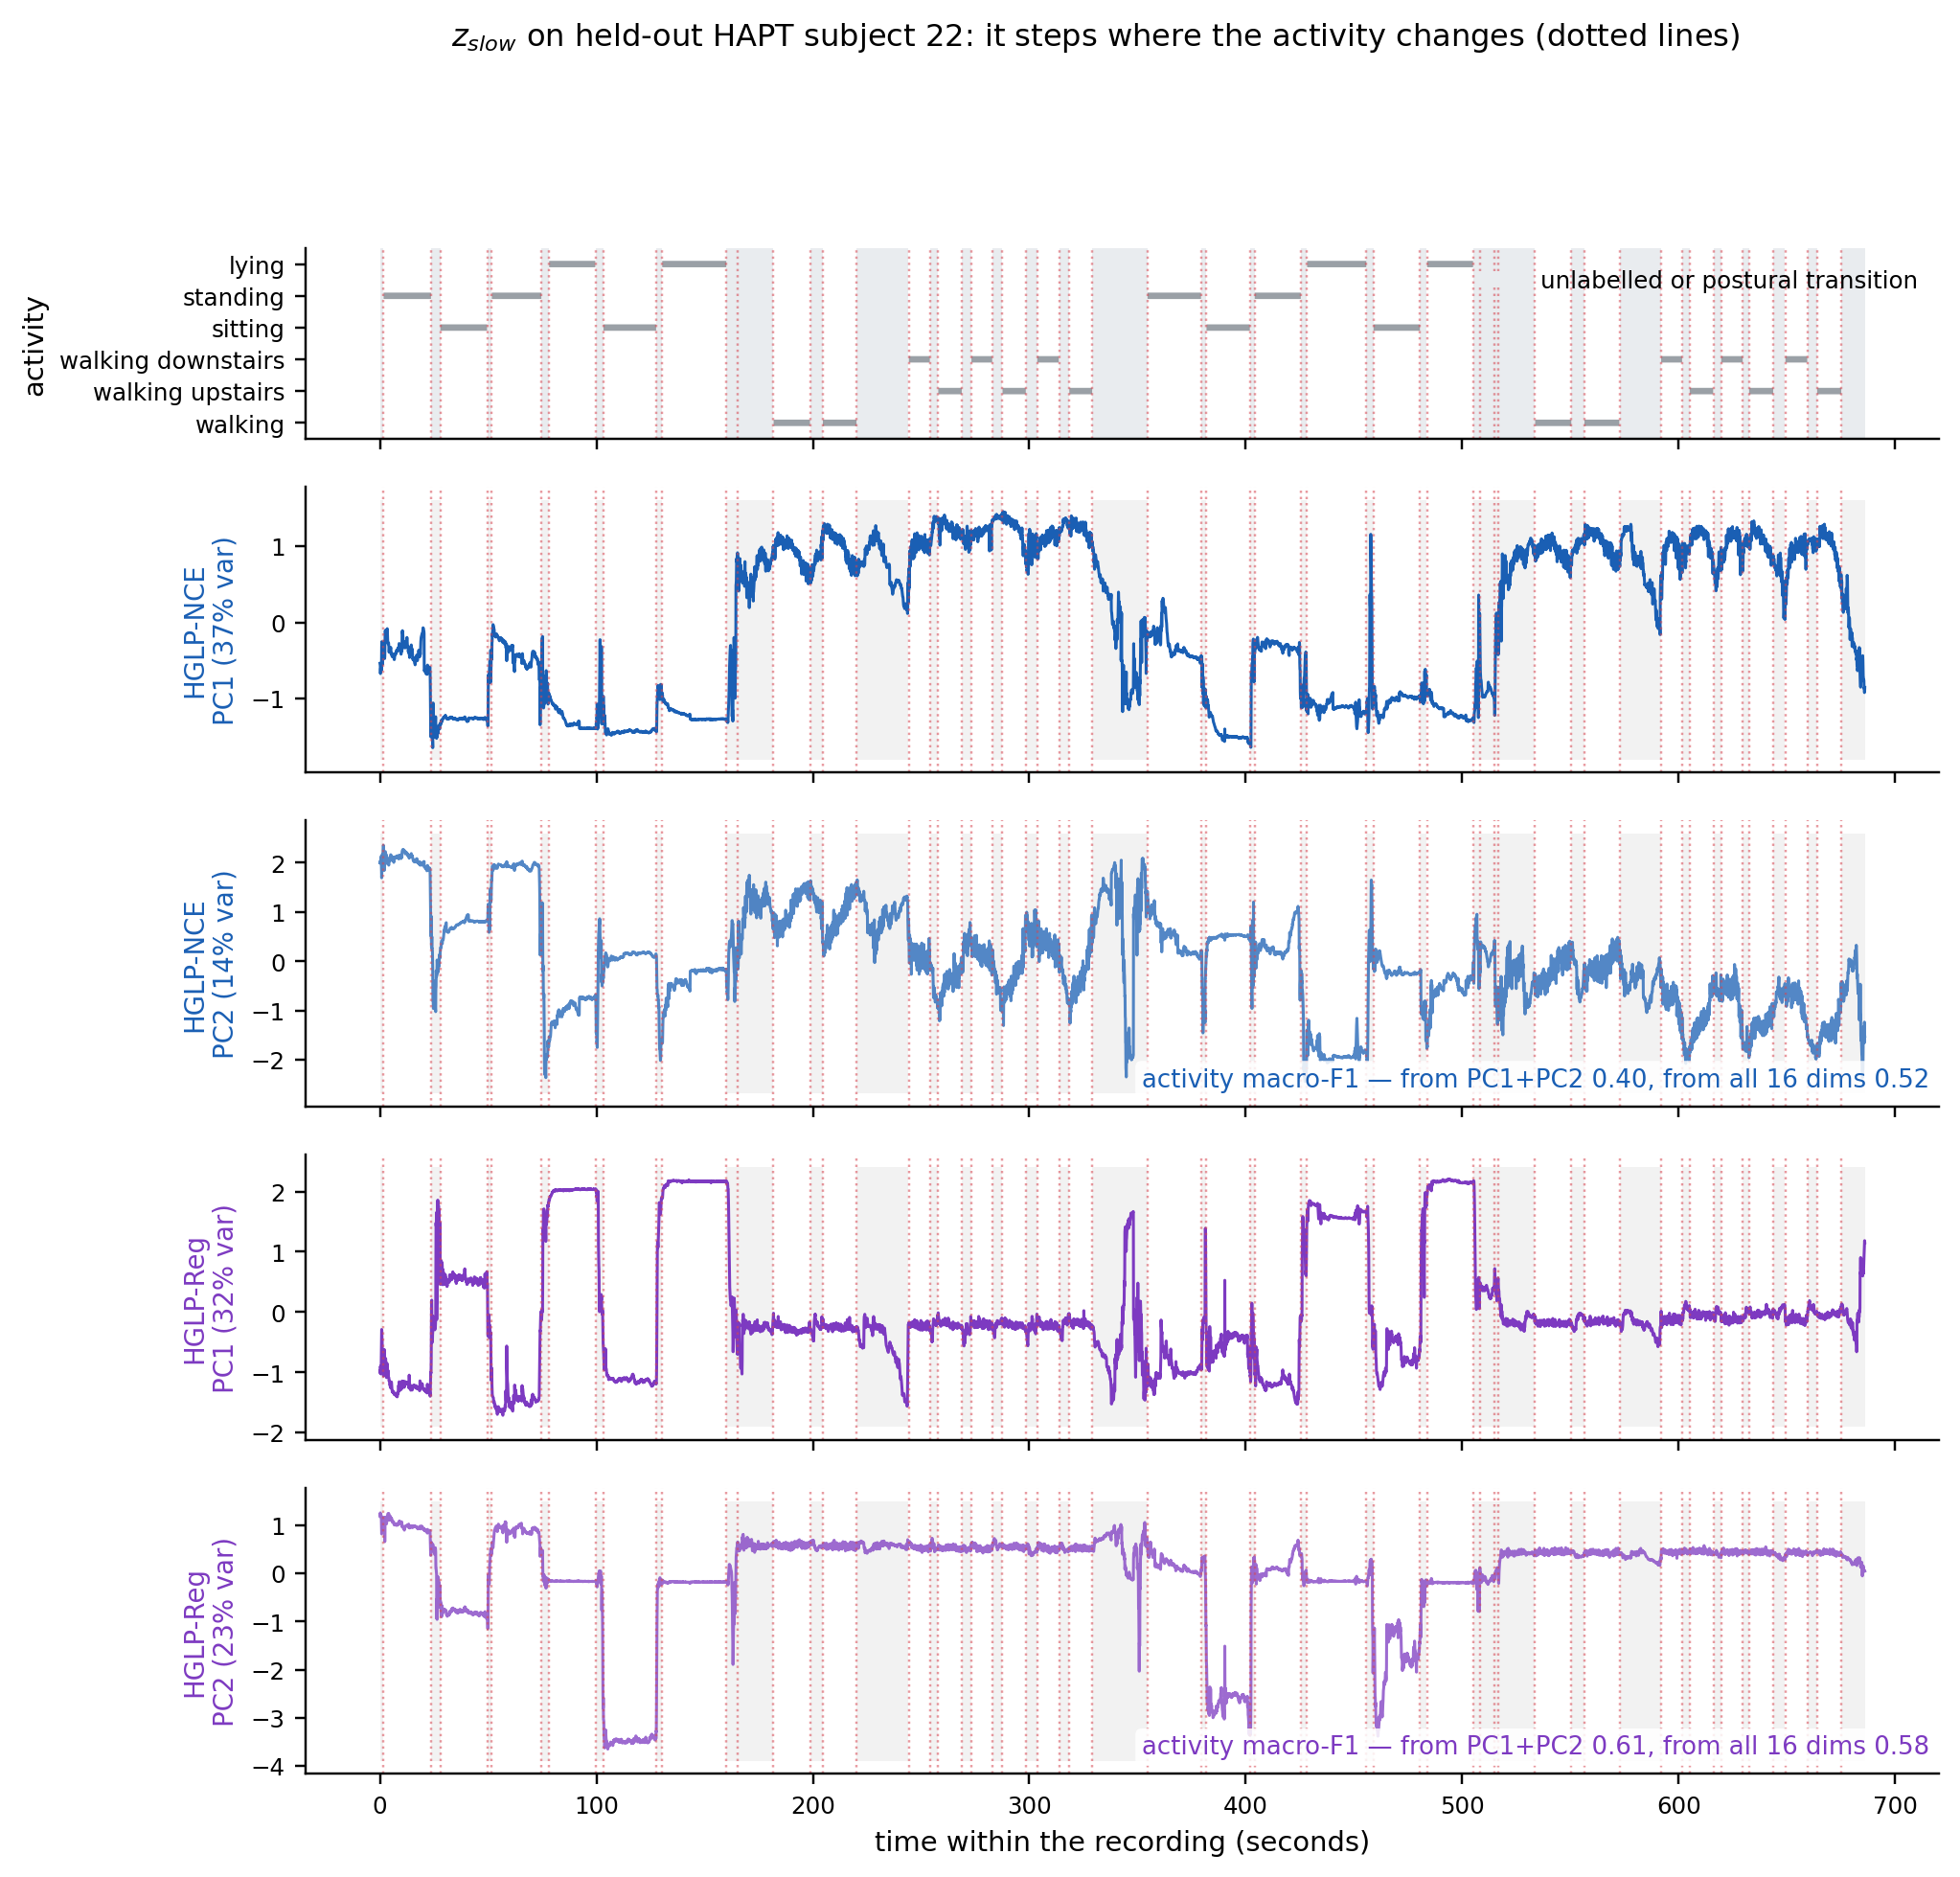
\includegraphics[width=0.9\textwidth]{figs/fig_traj_hapt.png}
\caption{$\zslow$ read as a trajectory rather than as classifier input (HAPT). Using the separated block this way needs no labels at evaluation time and no probe, which is the use the downstream cost of Section~\ref{sec:cost} is paid for; we report the figure and do not claim a quantitative result from it.}
\label{fig:traj}
\end{figure}
